\documentclass[aspectratio=169, 10pt]{beamer}

\usepackage{bm} % bold math
\usepackage{fontspec}
\usepackage{minted}
\usepackage{pgf-pie}
\usepackage{tikz}
\usepackage{graphicx}
\newcommand\sbullet[1][.5]{\mathbin{\vcenter{\hbox{\scalebox{#1}{$\bullet$}}}}}

% Custom commands and environments
\makeatletter
\newcommand\version[1]{\renewcommand\@version{#1}}
\newcommand\@version{}
\def\insertversion{\@version}

\newcommand\course[1]{\renewcommand\@course{#1}}
\newcommand\@course{}
\def\insertcourse{\@course}

\newcommand\coursetitle[1]{\renewcommand\@coursetitle{#1}}
\newcommand\@coursetitle{}
\def\insertcoursetitle{\@coursetitle}

\newcommand\lecturenumber[1]{\renewcommand\@lecturenumber{#1}}
\newcommand\@lecturenumber{}
\def\insertlecturenumber{\@lecturenumber}
\makeatother

\newcommand{\slidetitle}[1]{{\xbseries \large \structure{#1}} \bigskip}
\newcommand{\term}[1]{{\color{blue} #1}}
\newcommand{\leftspace}{\hspace{1em}}
\newcommand{\inlinearrow}{
  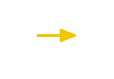
\begin{tikzpicture}[baseline]
    \node [anchor=base] (x) {};
    \draw [rawarrow] (x.mid west) -- ($(x.mid west) + (2em,0)$);
  \end{tikzpicture}
}

\newenvironment{slide}
{\begin{frame}[fragile,environment=slide]\vskip0pt plus 1filll}
{\vskip0pt plus 1filll\end{frame}}

% LaTeX

\setlength{\leftmargini}{1em}

% Common Information

\author{Talia Xu}
\course{COMPSCI 340}
\coursetitle{Operating Systems}
\date{2024 Semester 2}

% fontspec

\defaultfontfeatures{Ligatures=TeX}
% \setmainfont{Domine}
\setsansfont{Inter}[
  FontFace={ul}{n}{Font=*-Thin},
  FontFace={el}{n}{Font=*-ExtraLight},
  FontFace={l}{n}{Font=*-Light},
  FontFace={sb}{n}{Font=*-SemiBold},
  FontFace={eb}{n}{Font=*-ExtraBold},
  FontFace={xb}{n}{Font=*-Black},
]
\setmonofont[Contextuals=AlternateOff, Ligatures=TeXOff]{Iosevka}[
  FontFace={xb}{n}{Font=*-Heavy},
]

%% Font Weights

\DeclareRobustCommand{\ulseries}{\fontseries{ul}\selectfont}
\DeclareTextFontCommand{\textul}{\ulseries}
\DeclareRobustCommand{\elseries}{\fontseries{el}\selectfont}
\DeclareTextFontCommand{\textel}{\elseries}
\DeclareRobustCommand{\lseries}{\fontseries{l}\selectfont}
\DeclareTextFontCommand{\textl}{\lseries}
\DeclareRobustCommand{\sbseries}{\fontseries{sb}\selectfont}
\DeclareTextFontCommand{\textsb}{\sbseries}
\DeclareRobustCommand{\ebseries}{\fontseries{eb}\selectfont}
\DeclareTextFontCommand{\texteb}{\ebseries}
\DeclareRobustCommand{\xbseries}{\fontseries{xb}\selectfont}
\DeclareTextFontCommand{\textxb}{\xbseries}

% tikz

\usetikzlibrary{
  arrows,
  arrows.meta,
  automata,
  backgrounds,
  calc,
  decorations.pathreplacing,
  matrix,
  positioning,
  overlay-beamer-styles,
  shapes,
  shapes.multipart,
  tikzmark,
}

\tikzstyle{rawarrow} = [
  -{Latex[round]},
  line width=1pt,
  yellow,
  shorten >=3pt,
  shorten <=3pt,
  font=\small,
  text=black,
]

\tikzstyle{arrow} = [
  -{Latex[round]},
  line width=1pt,
  yellow,
  shorten >=3pt,
  shorten <=3pt,
  transform canvas={yshift=3pt},
  font=\small,
  text=black,
]

\newcommand{\tikzmarkcoord}[1]{([yshift=3pt]pic cs:#1)}

% minted

\setminted{style=eyolfson, fontsize=\small, escapeinside=||}
\setmintedinline{fontsize=\normalsize}

% hyperref

\hypersetup{colorlinks, urlcolor=blue}

% beamer
\setbeamersize{text margin left=16mm, text margin right=16mm}
\setbeamertemplate{itemize items}[circle]
\setbeamercolor{item}{fg=black}
\setbeamercolor{structure}{fg=darkblue}
\setbeamerfont{frametitle}{series=\bfseries, parent=structure}
\setbeamertemplate{navigation symbols}{}
\setbeamertemplate{headline}{}
\setbeamertemplate{footline}{
  \begin{tikzpicture}[
    remember picture,
    overlay,
    shift={(current page.south west)},
  ]
    \path [fill=gray] (144mm, 0) -- (160mm, 16mm) -- (160mm, 0);
    \node [inner sep=3.5mm, outer sep=0, text=black, anchor=base east,
           align=right, yshift=3.5mm]
          at (current page.south east) {\ttfamily \small \insertframenumber{}};
  \end{tikzpicture}
}
\setbeamertemplate{title page}{
  \begin{tikzpicture}[
    remember picture,
    overlay,
    shift={(current page.south west)},
    background rectangle/.style={fill=darkblue},
    show background rectangle,
  ]
    \node [anchor=center, align=center, text=white, text width=40mm, scale=3.2]
          at (\paperwidth / 2, \paperheight * 2 / 3)
          {\xbseries \inserttitle{}};
    \node [anchor=base west, align=left, inner sep=0, text=white, yshift=2.5mm]
          at (16mm, \paperheight / 3)
          {\insertdate{} \insertcourse{}: \insertcoursetitle{}};
    \node [anchor=base west, align=left, inner sep=0, text=white, yshift=-2.5mm]
          at (16mm, \paperheight / 3)
          {\insertauthor};
    \node [anchor=base east, align=right, inner sep=0, text=white, yshift=2.5mm]
          at (144mm, \paperheight / 3)
          {Lecture \insertlecturenumber{}};
    \node [anchor=base east, align=right, inner sep=0, text=white,
           yshift=-2.5mm]
          at (144mm, \paperheight / 3)
          {\ttfamily \insertversion{}};
    \node [align=center, anchor=south, inner sep=0, text=white, yshift=3.5mm]
          (license) at (\paperwidth / 2, 0)
          {\fontsize{7pt}{7pt}\selectfont This  work is licensed under a
           \href{http://creativecommons.org/licenses/by-sa/4.0/}
                {\color{lightblue} Creative Commons Attribution-ShareAlike 4.0
                 International License}};
  \end{tikzpicture}
}

% xcolor

%% Primary Colour

\definecolor{pantone655}{RGB}{0, 42, 92} % #002a5c
\colorlet{darkblue}{pantone655}

%% Secondary Colours

\definecolor{pantone633}{RGB}{0, 139, 176} % #008bb0
\colorlet{blue}{pantone633}

\definecolor{pantonewarmred}{RGB}{220, 70, 51} % #dc4633
\colorlet{red}{pantonewarmred}

\definecolor{pantone3285}{RGB}{0, 161, 137} % #00a189
\colorlet{cyan}{pantone3285}

\definecolor{pantone7722}{RGB}{13, 83, 77} % #0d534d
\colorlet{darkcyan}{pantone7722}

\definecolor{pantone376}{RGB}{141, 191, 46} % #8dbf2e
\colorlet{green}{pantone376}

\definecolor{pantone2613}{RGB}{109, 36, 122} % #6d247a
\colorlet{violet}{pantone2613}

\definecolor{pantone2985}{RGB}{111, 199, 234} % #6fc7ea
\colorlet{lightblue}{pantone2985}

\definecolor{pantone227}{RGB}{171, 19, 104} % #ab1368
\colorlet{magenta}{pantone227}

\definecolor{pantone7406}{RGB}{241, 197, 0} % #f1c500
\colorlet{yellow}{pantone7406}

%% Neutrals

\definecolor{pantonecoolgray2}{RGB}{208, 209, 201} % #d0d1c9
\colorlet{gray}{pantonecoolgray2}


\lecturenumber{28}
\title{inodes}
\version{2.0.0}

\begin{document}

  \begin{frame}[plain, noframenumbering]
    \titlepage
  \end{frame}

  \begin{slide}
    
    \slidetitle{
      An inode Describes a File System Object
    
      (Files and Directories)
    }

    \includegraphics[height=0.8\textheight]{hinode.png}

  \end{slide}

  \begin{slide}
    
    \slidetitle{
      inodes Aim to Be Efficient for Small Files,
      
      and Support Large Ones
    }

    UNIX inodes hold metadata and pointers to blocks
    \medskip

    Smaller files only use direct pointers
    \medskip

    Larger files have additional index nodes with pointers to additional blocks
    \medskip

    Very small files can have its contents directly inside the inode

  \end{slide}

  \begin{slide}
    
    \slidetitle{inode Problem}
    
    Assume this scenario:

    \begin{itemize}
      \item An index block stores 12 direct pointers, 1 single, double and
            triple indirect pointer each
      \item A disk block is 8~KiB in size
      \item A pointer to a block is 4~Bytes
      \item Indirect blocks consist of direct pointers only
    \end{itemize}
    \medskip

    What is the maximum size of a file managed by this index block?

  \end{slide}

  \begin{slide}
    
    \slidetitle{inode Solution}
    
    Assume this scenario:

    \begin{itemize}
      \item An index block stores 12 direct pointers, 1 single, double and triple indirect pointer each
      \item A disk block is 8~KiB in size
      \item A pointer to a block is 4~Bytes
      \item Indirect blocks consist of direct pointers only
    \end{itemize}
    \medskip

    \# pointers per indirect table = $\mathsf{\frac{2^{13}}{2^2} = 2^{11}}$

    \# addressable blocks = $\mathsf{12 + 2^{11} + (2^{11})^2 + (2^{11})^3 \approx (2^{11})^3 = 2^{33}}$

    Total of bytes = $\mathsf{2^{33} * 2^{13} = 2^{46} = 64 TiB}$

  \end{slide}

  \begin{slide}
    
    \slidetitle{Hard Links Are Pointers to inodes}

    \begin{center}
      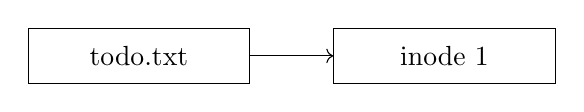
\begin{tikzpicture}[node distance=0mm and 0mm]

        \node[rectangle,draw,minimum width=80,minimum height=20] (inode1)   {inode 1};
        \node[rectangle,draw,minimum width=80,minimum height=20,xshift=-30] (fileA)  [left=of inode1] {todo.txt};

        \draw[->] (fileA.east) -- (inode1.west);

      \end{tikzpicture}
    \end{center}
    \medskip

    A directory entry (aka filename) is called a \textit{hard link}
    \medskip

    A hard link points to one inode

  \end{slide}

  \begin{slide}
    
    \slidetitle{Multiple Hard Links Can Point to the Same inode}

    \begin{center}
      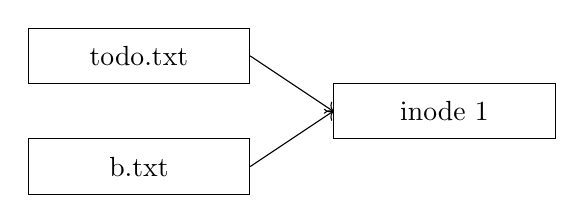
\begin{tikzpicture}[node distance=0mm and 0mm]

        \node[rectangle,draw,minimum width=80,minimum height=20] (inode1)   {inode 1};
        \node[rectangle,draw,minimum width=80,minimum height=20,xshift=-30,yshift=20] (fileA)  [left=of inode1] {todo.txt};
        \node[rectangle,draw,minimum width=80,minimum height=20,xshift=-30,yshift=-20] (fileB)  [left=of inode1] {b.txt};

        \draw[->] (fileA.east) -- (inode1.west);
        \draw[->] (fileB.east) -- (inode1.west);

      \end{tikzpicture}
    \end{center}
    \medskip

    Deleting a file only removes a hard link
    
    \leftspace{}(the file can be hard liked somewhere else)
    \medskip

    POSIX has the \texttt{unlink} call rather than a delete call

  \end{slide}

  \begin{slide}
    
    \slidetitle{Soft Links Are Paths to Another File}

    \begin{center}
      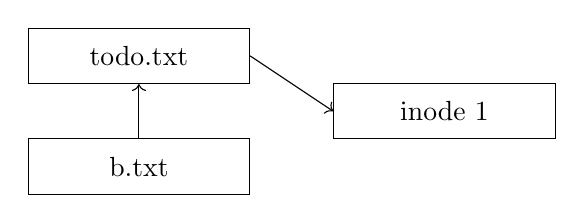
\begin{tikzpicture}[node distance=0mm and 0mm]

        \node[rectangle,draw,minimum width=80,minimum height=20] (inode1)   {inode 1};
        \node[rectangle,draw,minimum width=80,minimum height=20,xshift=-30,yshift=20] (fileA)  [left=of inode1] {todo.txt};
        \node[rectangle,draw,minimum width=80,minimum height=20,xshift=-30,yshift=-20] (fileB)  [left=of inode1] {b.txt};

        \draw[->] (fileA.east) -- (inode1.west);
        \draw[->] (fileB.north) -- (fileA.south);

      \end{tikzpicture}
    \end{center}
    \medskip

    When resolving the file, the file system is redirected somewhere else, so:
    \begin{itemize}
      \item Soft link targets do not need to exist
      \item Soft link targets can be deleted without notice of the soft link
      \item Unresolvable soft links lead to an exception
    \end{itemize}

  \end{slide}

  \begin{slide}
    
    \slidetitle{Filesystem Example Problem}

    \begin{minted}{console}
touch todo.txt
ln todo.txt b.txt
ln -s todo.txt c.txt
mv todo.txt d.txt
rm b.txt
    \end{minted}
    \medskip

    How does the FS look like before and after the mv and rm commands?

  \end{slide}

  \begin{slide}
    
    \slidetitle{Filesystem Example Solution (1)}

    \begin{minted}{console}
touch todo.txt
ln todo.txt b.txt
ln -s todo.txt c.txt
mv todo.txt d.txt
rm b.txt
    \end{minted}
    \medskip

    Before mv:
    \medskip

    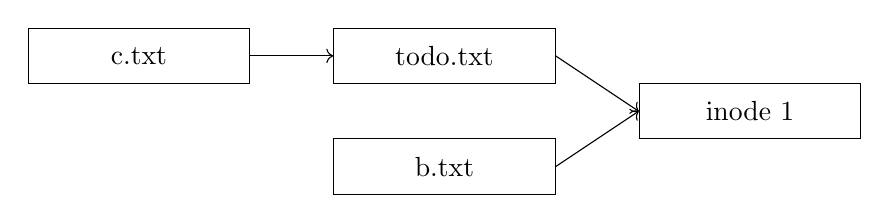
\begin{tikzpicture}[node distance=0mm and 0mm]
      \node[rectangle,draw,minimum width=80,minimum height=20] (inode1)   {inode 1};
      \node[rectangle,draw,minimum width=80,minimum height=20,xshift=-30,yshift=20] (fileA)  [left=of inode1] {todo.txt};
      \node[rectangle,draw,minimum width=80,minimum height=20,xshift=-30,yshift=-20] (fileB)  [left=of inode1] {b.txt};
      \node[rectangle,draw,minimum width=80,minimum height=20,xshift=-30] (fileC)  [left=of fileA] {c.txt};
  
      \draw[->] (fileA.east) -- (inode1.west);
      \draw[->] (fileB.east) -- (inode1.west);
      \draw[->] (fileC.east) -- (fileA.west);
    \end{tikzpicture}

  \end{slide}

  \begin{slide}
    
    \slidetitle{Filesystem Example Solution (2)}

    \begin{minted}{console}
touch todo.txt
ln todo.txt b.txt
ln -s todo.txt c.txt
mv todo.txt d.txt
rm b.txt
    \end{minted}
    \medskip

    After mv:
    \medskip

    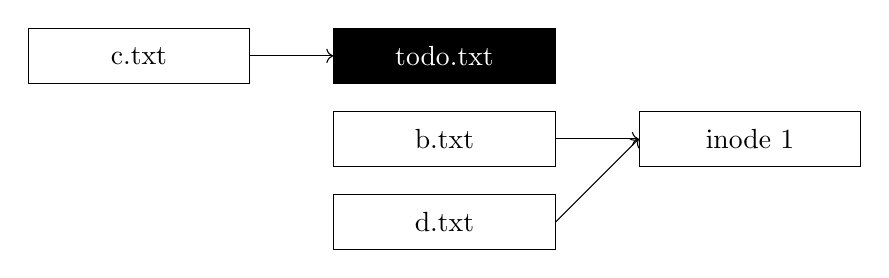
\begin{tikzpicture}[node distance=0mm and 0mm]

      \node[rectangle,draw,minimum width=80,minimum height=20] (inode1)   {inode 1};
      \node[rectangle,draw,minimum width=80,minimum height=20,xshift=-30,yshift=30,fill=black,text=white] (fileA)  [left=of inode1] {todo.txt};
      \node[rectangle,draw,minimum width=80,minimum height=20,xshift=-30] (fileB)  [left=of inode1] {b.txt};
      \node[rectangle,draw,minimum width=80,minimum height=20,xshift=-30,yshift=-30] (fileD)  [left=of inode1] {d.txt};
      \node[rectangle,draw,minimum width=80,minimum height=20,xshift=-30] (fileC)  [left=of fileA] {c.txt};
  
      \draw[->] (fileD.east) -- (inode1.west);
      \draw[->] (fileB.east) -- (inode1.west);
      \draw[->] (fileC.east) -- (fileA.west);
    \end{tikzpicture}

  \end{slide}

  \begin{slide}
    
    \slidetitle{Filesystem Example Solution (3)}

    \begin{minted}{console}
touch todo.txt
ln todo.txt b.txt
ln -s todo.txt c.txt
mv todo.txt d.txt
rm b.txt
    \end{minted}
    \medskip

    After rm:
    \medskip

    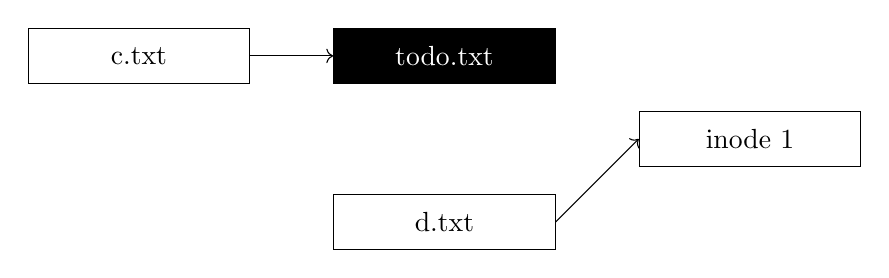
\begin{tikzpicture}[node distance=0mm and 0mm]

      \node[rectangle,draw,minimum width=80,minimum height=20] (inode1)   {inode 1};
      \node[rectangle,draw,minimum width=80,minimum height=20,xshift=-30,yshift=30,fill=black,text=white] (fileA)  [left=of inode1] {todo.txt};
      \node[rectangle,draw,minimum width=80,minimum height=20,xshift=-30,yshift=-30] (fileD)  [left=of inode1] {d.txt};
      \node[rectangle,draw,minimum width=80,minimum height=20,xshift=-30] (fileC)  [left=of fileA] {c.txt};
    
      \draw[->] (fileD.east) -- (inode1.west);
      \draw[->] (fileC.east) -- (fileA.west);
    
    \end{tikzpicture}

  \end{slide}

  \begin{slide}
    
    \slidetitle{In UNIX, Everything is a File}

    Directories are files of type ``directory''
    \medskip

    Additional types are:
    
    \leftspace{}``regular file'', ``block device'' (HDDs, SSDs),
    ``pipe'', ``socket'' etc.
    \medskip

    Directory inodes do not store pointers to data blocks
    
    \leftspace{}but rather filenames and pointers to inodes

  \end{slide}

  \begin{slide}
    
    \slidetitle{What Data is Stored in an inode?}
     \small
      \begin{itemize}
        \item[a] Filename
        \item[b] Containing Directory name
        \item[c] File Size 
        \item[d] File type
        \item[e] \# of soft links to file
        \item[f] location of soft links 
        \item[g] \# of hard links to file  
        \item[h] location of hard links
        \item[i] access rights
        \item[j] timestamps
        \item[k] file contents
        \item[l] ordered list of data blocks     
      \end{itemize}
  \end{slide}

  \begin{slide}
    
    \slidetitle{What Data is Stored in an inode? Solution}
     \small
      \begin{itemize}
        \item[a] Filename \textit{No. Names are stored in directories}
        \item[b] Containing Directory name \textit{No. File can be in multiple dirs}
        \item[c] File Size \textit{Yes}
        \item[d] File type \textit{Yes}
        \item[e] \# of soft links to file \textit{No (they are unknown)}
        \item[f] location of soft links \textit{No (they are unknown)}
        \item[g] \# of hard links to file \textit{Yes (to know when to erase the file, check \texttt{stat})}
        \item[h] location of hard links \textit{No (they are unknown to the inode)}
        \item[i] access rights \textit{Yes}
        \item[j] timestamps \textit{Yes}
        \item[k] file contents \textit{Sometimes}
        \item[l] ordered list of data blocks \textit{Yes, by definition} 
      \end{itemize}
  \end{slide}

  \begin{slide}
    
    \slidetitle{Filesystem Caches Speed Up Writing to Disks}

    Writing data to the disk is slow, we can use a cache to speed it up
    \medskip

    File blocks are cached in main memory in the \textit{filesystem cache}
    
    \leftspace{}Referenced blocks are likely to be referenced again (temporal locality)

    \leftspace{}Logically near blocks are likely to be referenced (spatial locality)
    \medskip

    A kernel thread (or daemon) writes changes periodically to disk
    \medskip
    
    \texttt{flush} and \texttt{sync} system calls trigger a permanent write

  \end{slide}

  \begin{slide}
    
    \slidetitle{Journaling Filesystem}

    Deleting a file on a Unix file system involves three steps:

    \begin{enumerate}
      \item Removing its directory entry.
      \item Releasing the inode to the pool of free inodes.
      \item Returning all disk blocks to the pool of free disk blocks.
    \end{enumerate}
    \medskip

    Crashes could occur between any steps, leading to a storage leak
    \medskip

    The journal contains operations in progress,
    
    \leftspace{}so if a crash occurs we can recover

  \end{slide}

  \begin{slide}
    
    \slidetitle{inodes Are a Hybrid Allocaiton Strategy}
    
    inodes are offer greater flexibility over: contiguous, linked, FAT, or
    indexed

    \begin{itemize}
      \item Everything is a file on UNIX, names in a directory can be hard or
            soft links
    \end{itemize}

  \end{slide}

\end{document}
